% $Id: loadproject.tex 6092 2007-11-27 13:25:32Z alexandra $
% Local Variables:
% ispell-check-comments: nil
% Local IspellDict: american
% End:
% --------------------------------------------------------
% User documentation
% copyright by BREDEX GmbH 2005
% --------------------------------------------------------

\index{Project!Open}
\index{Open Project}

\begin{enumerate}
\item To open a \gdproject{} from the database, select:\\
\bxmenu{Project}{Open}{}{}. 
\item If you haven't already logged into the database, a dialog will appear to ask you to do so.  See the previous section \bxpref{dblogin} for details. 
\item Choose the \gdproject{} you want to open from the combo box in the dialog which appears (\bxfigref{loadfromdb}). 

\begin{figure}
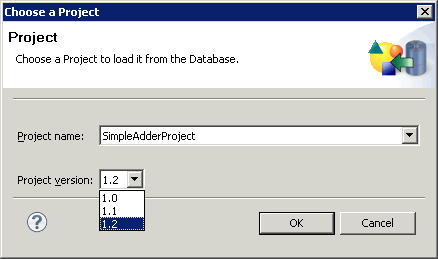
\includegraphics{Tasks/Projects/PS/loadfromdb}
\caption{Open \gdproject{} from \gddb{}}
\label{loadfromdb}
\end{figure}

\item If the \gdproject{} has more than one version, choose which version you want to open. For more information on \gdproject{} versions, see the section later \bxpref{projectversion}. 
\item The \gdproject{} is opened in the client. 
\end{enumerate}



  
